\documentclass{mldsmsc}
% \setlength{\parindent}{20pt}

\title{Probabilistic Sequential Matrix Factorisation for 12-lead \\ ECG Data}
\author{Joana Levtcheva}
\CID{01252821}
\supervisor{Dr Deniz Akyildiz}
% \date{1 May 2023}
%For today's date, use:
\date{\today}
\logoimg{}


% THIS IS WHERE NEW COMMANDS CAN BE DEFINED
% commands below only used in the proof; otherwise can be deleted
\newcommand{\consta}{a}
\newcommand{\X}{X}
\newcommand{\EE}[1]{ \mathrm{E} [ #1 ] }
\newcommand{\inparenth}[1]{\left( #1 \right)}

\begin{document}

% Generates the Title Page
\maketitle


% Generates plagiarism declaration
\declarationname{Joana Levtcheva}
\declarationdate{\today}
\declaration 

\begin{abstract}

Matrix factorisation (MF) techniques are highly effective and widely used in unsupervised machine learning. By decomposing the original matrix into multiple simpler lower-dimensional matrices, MF aims to uncover latent structures that are not immediately obvious in the original matrix. MF finds applications in areas such as image processing, natural language processing, missing data imputation, and recommendation systems. Despite considerable progression in the probabilistic versions, there is demand for such methods in applications such as uncertainty quantification, managing time-series data, and executing efficient probabilistic components. \newline

\noindent In this thesis, we show novel applications of the probabilistic sequential MF algorithm Probabilistic Sequential Matrix Factorisation (PSMF) (\cite{akyildiz2021probabilistic}) to 12-lead ECG data. We explore three tasks related to this complex high-dimensional time-series data with nonlinear subspace: missing data imputation with PSMF and the robust version of PSMF (rPSMF) (\cite{akyildiz2021probabilistic}) and compare their performance with other probabilistic sequential MF algorithms, R-peaks detection, and forecasting an ECG component based on previous normal heart beats using a Fourier basis with multiple terms and rank higher than one. We perform our experiments using the high-quality comprehensive dataset "A Large Scale 12-lead Electrocardiogram Database for Arrhythmia Study" (\cite{cite1}, \cite{cite2}, \cite{cite3}). We describe and outline the experimenting process and the challenges we encountered modelling the complex ECG data, and summarise the experiments results. We find that PSMF performs well when used for imputing missing data, but when it comes to forecasting there are certain challenges which open the door for further research on extending the PSMF algorithm to better handle the complex structure of ECG data. \newline

\end{abstract}

\begin{acknowledgements}

TODO 

\end{acknowledgements}

% add glossary?

% table of contents
\tableofcontents

% VERY IMPORTANT
% This command switches from Roman to Arabic numbering for main part of thesis
\mainmatter


\chapter{Introduction}

Matrix factorisation (or also matrix decomposition) in the context of linear algebra is simply a factorisation of a matrix into a product of multiple matrices. Many different decompositions exist, and they find various applications in mathematical problems such as solving systems of linear equations, matrix inversion, determinant computation, eigenvalues problems, solving systems of first order ODEs, etc. \newline

\noindent In this thesis, we are interested in matrix factorisation (MF) in the context of machine learning. Nowadays, MF techniques are highly effective and widely used in unsupervised machine learning. These methods aim to decompose the original matrix into multiple lower-dimensional matrices. By breaking the matrix into these simpler components MF aims to uncover latent structures that are not immediately apparent in the original matrix. Some applications are in image processing: for reducing dimensionality and noise in images, NLP for topic modelling, missing data imputation, recommendation systems, etc. \newline

\noindent Formally, we are interested in the general problem of factorising a data matrix $Y \in \mathbb{R}^{m \times n}$ as

\begin{equation}
Y \approx CX,
\end{equation} \newline
\noindent where $C \in \mathbb{R}^{m \times r}$ is the \textit{dictionary matrix}, $X \in \mathbb{R}^{r \times n}$ is the \textit{coefficients matrix} (with columns the coefficients), and $r$ is the \textit{approximation rank} (\cite{cite-key}). Visually we can present the problem as

\begin{equation}
\underbrace{
\begin{bmatrix}
  \times & \times & \times & \times & \times \\
  \times & \times & \times & \times & \times \\
  \times & \times & \times & \times & \times
\end{bmatrix}
}_{\text{Y $\in \mathbb{R}^{m \times n}$ }}
\approx
\underbrace{
\begin{bmatrix}
  \times & \times \\
  \times & \times \\
  \times & \times
\end{bmatrix}
}_{\text{C $\in \mathbb{R}^{m \times r}$ }}
\underbrace{
\begin{bmatrix}
  \times & \times & \times & \times & \times \\
  \times & \times & \times & \times & \times
\end{bmatrix}
}_{\text{X $\in \mathbb{R}^{r \times n}$ }}.
\end{equation}

\noindent There are also probabilistic versions of MF which incorporate probabilistic models to better handle uncertainty and variability in the data, leading to more accurate predictions. Such methodologies postulate a prior distribution over the latent factors and necessitate the computation of the posterior distribution to derive updated estimates. With that the matrix is not only decomposed but probabilistic interpretations of the factors are also possible. \newline

\noindent We should also note that some algorithms are suitable for sequential data - updating $C$ and $X$ incrementally as new data points are observed and thus incorporating temporal dynamics and sequential dependencies into the factorisation process, and others are non-sequential - treating the dataset as a batch, independent of the time varying component. \newline

\noindent Throughout this thesis we are going to focus on probabilistic sequential MF algorithms, along with their application to 12-lead ECG data, targeting the problem of managing high-dimensional time-series data with nonlinear subspace. Some examples of probabilistic MF algorithms are Probabilistic Matrix Factorisation (PMF) (\cite{NIPS2007_d7322ed7}) - non-sequential, Dictionary filtering (\cite{cite-key}), Probabilistic Sequential Matrix Factorization (PSMF) (\cite{akyildiz2021probabilistic}). \newline

\noindent The paper "Probabilistic matrix factorisation" (PMF) (\cite{NIPS2007_d7322ed7}) introduces an efficient and scalable probabilistic model for collaborative filtering. The algorithm performs well on large, sparse and imbalanced datasets. This is demonstrated by using a Netflix dataset, where PMF models the user preference matrix $R$ as a product of two lower-dimensional matrices: user feature matrix $U$ and movie feature matrix $V$. The conditional distribution over observed ratings is modeled using Gaussian noise, and zero-mean spherical Gaussian priors are placed on the user and movie feature vectors. The paper also presents two extensions to the initial PMF model: incorporating \textit{adaptive priors} to automatically control the model complexity through these priors over the model parameters, and a \textit{constrained PMF} version to handle and improve predictions for users with few ratings by incorporating constraints based on the assumption that users with similar movie ratings have similar preferences. The authors show that PMF significantly outperforms traditional Singular Value Decomposition (SVD) (\cite{4ba978eb-d878-342d-a11e-6d7554474b2d}) models and scales linearly with the number of observations. It's worth noting that PMF treats each rating as an independent event meaning the time varying component is not taken into consideration, making PMF a batch learning model designed to process large datasets in a non-sequential manner. \newline

\noindent Later, in the paper "Dictionary Filtering: A Probabilistic Approach to Online Matrix Factorization" (DF) (\cite{cite-key}), the authors introduce a novel online MF algorithm known as dictionary filtering. It leverages probabilistic models, specifically using recursive linear filters, and efficiently factorises the original data matrix into a dictionary matrix and a coefficients matrix. This is an online and sequential algorithm, meaning it is suitable for high-dimensional and time-varying data, and it also has easy to tune parameters. DF is efficient for high-dimensional data with its computational complexity of $O(mr^2)$ independent of the number of data points. Although the model can learn non-stationary and dynamic data, it is developed for linear and Gaussian state space models (SSM). Particularly for ECG data, ECG has a nonlinear SSM which doesn't suit the dictionary filtering. \newline

\noindent Two years later, Akyildiz et.al. develop Probabilistic Sequential Matrix Factorization (PSMF) (\cite{akyildiz2021probabilistic}). This method is tailored to time-varying and non-stationary datasets consisting of high-dimensional time-series. Nonlinear Gaussian SSMs are considered, decomposing the original matrix into a dictionary matrix and time-variying coefficient matrix. This time, the matrices are with potentially nonlinear dependencies, with PSMF efficiently capturing temporal dependencies through Markovian structures on the coefficients, making it possible to encode the dependencies into a lower dimensional latent space. The model is demonstrated to work on tasks such as forecasting, changepoint detection, missing data imputation, and is shown to work on real-world data with a periodic subspace. There is also a robust version rPSMF using Student-t filters to handle model misspecification, and a version for imputing missing data. Although the model is suitbale for reducing high-dimensional data with periodic subspaces to lower-dimensional latent space, PSMF might struggle with very large datasets, having many data points. \newline

% \noindent In the unpublished MSc thesis (Imperial College London) of Rina Maletta (\cite{rina}), the author introduces Matrix-Variate Gaussian Matrix Factorization (MVGMF). This is a novel PMF method using matrix-variate Gaussian distributions. The algorithm has fast Gaussian updates which take the form of a preconditioned MF algorithm which is stable. An extension for handling missing data and data imputation is also proposed. The method is tested on the Netflix Prize dataset, London air quality (NO2) data, and Olivetti face image dataset.

\section{Contributions}

Using probabilistic methods, and specifically probabilistic sequential MF ones, on ECG data is not widely explored. Hence, we aim to introduce a few novel real-world applications of the PSMF method to 12-lead ECG data. The contributions made in this thesis are:

\begin{itemize}
    \item We show three novel applications of PSMF to complex 12-lead ECG data.
    \item Application 1: We apply both PSMF and rPSMF for imputing missing data in the ECG signals, and compare the results with other sequential probabilistic MF models.
    \item Application 2: We show that PSMF can be used for R-peaks detection by introducing a simple approach. We remove the reconstructed signal, which has modelled the R-peaks smoother than the real ones, from the original data, and determine a suitable threshold for selecting the peaks. 
    \item Application 3: We forecast an ECG component based on previous normal heart beats by incorporating a Fourier basis with multiple Fourier terms and rank higher than 1. 
    % We experiment with the original high quality data with many points, as well as with a subsample of the data, defining the ECG signals with lower frequency. We also experiment with smoothing the data, standardising it and/or normalising it. We make conclusions based on the done analysis and comparison of performance and results.
\end{itemize}

\section{Notation}

We are going to denote the original data matrix as $Y$, and let $Y \in \mathbb{R}^{m \times n}$. Let $C \in \mathbb{R}^{m \times r}$ be the dictionary matrix, $X \in \mathbb{R}^{r \times n}$ be the coefficients matrix, and $r$ be the approximation rank. \newline

\noindent With $I_d \in \mathbb{R}^{d \times d}$ we are going to denote the identity matrix, with $MN(X; M, U, V)$ the matrix normal distribution with $M$ the mean-matrix, $U$ the row-covariance, and $V$ the column covariance. Further, with $N(x; \mu, \Sigma)$  let's denote the Gaussian density with mean $\mu$ and $\Sigma$ the covariance matrix, $IG(s; \alpha, \beta)$ is the inverse gamma distribution with shape $\alpha$ and scale $\beta$.  \newline

\noindent TODO:

\begin{itemize}
    \item the mapping $f_\theta$
    \item vectorisation
    \item multivariate normal distribution
\end{itemize}

% \noindent  We denote the vectorised forms of the matrices with their respective lower case letters. We can formally define c = vec(C), where vec(·) is the vectorisation operation. The columns of C are stacked on each other, so if C ∈ Rm×r, then c ∈ Rmr×1. We can also define the inverse vectorisation operator C = vec−1(c). \newline

% \noindent We have that p(x) denotes the probability density function (pdf) of x and p(y|x) is the conditional density of y given x. Where A ∈ Rm×n is a matrix, then MN(A;M,U, V ) denotes the matrix normal pdf for A, where M ∈ Rm×n is the mean, U ∈ Rn×n is the among-row co-variance and V ∈ Rm×m is the among-column co-variance. We also define the multivariate normal distribution in the following way; let a ∈ Rm, then N(a; μ, Σ) denotes the pdf of the multivariate normal distribution for the random variable a, where μ ∈ Rm is the mean and Σ ∈ Rm×m is the covariance matrix. Im ∈ Rm×m is the m×m identity matrix. \newline

\chapter{Background}

\section{Preliminaries}

\subsection{Matrix Normal Distribution} 

TODO 

\subsection{Kronecker Product}

\begin{definition}
Let $A \in \mathbb{R}^{m \times n}$ and $B \in \mathbb{R}^{p \times q}$ be matrices. Then their \textit{Kronecker product} denoted as $A \otimes B \in \mathbb{R}^{mp \times nq}$ is given by (\cite{alma993596394401591})

\begin{equation}
    A \otimes B = \begin{bmatrix}
        a_{11}B & a_{12}B & \hdots & a_{1n}B \\
        a_{21}B & a_{22}B & \hdots & a_{2n}B \\
        \vdots & \vdots & \ddots & \vdots \\
        a_{m1}B & a_{m2}B & \hdots & a_{mn}B
    \end{bmatrix},
\end{equation}
where $\{a_{ij}\}$, $i \in \{1,...,m\}$, $j \in \{1, ..., n\}$ are the elements of $A$.
\end{definition}

\subsection{Fourier Series}

TODO

\section{PSMF}

Intro

\subsection{Model}

For observations $(y_k)_{k \geq 1} \in \mathbb{R}^{m}$, latent coefficients $(x_k)_{k \geq 1} \in \mathbb{R}^{r}$, and a dictionary matrix $C \in \mathbb{R}^{m \times r}$ the PSMF model can be described with the following state-space equations:

\begin{equation} \label{eq:1}
    p(C) = \mathcal{MN}(C; C_0, I_d, V_0)
\end{equation}
\begin{equation} \label{eq:2}
    p(x_0) = \mathcal{N}(x_0; \mu_0, P_0)
\end{equation}
\begin{equation} \label{eq:3}
    p_{\theta}(x_k \mid x_{k-1}) = \mathcal{N}(x_k; f_{\theta}(x_{k-1}), Q_k)
\end{equation}
\begin{equation} \label{eq:4}
    p(y_k \mid x_k, C) = \mathcal{N}(y_k; Cx_k, R_k)
\end{equation}

\noindent where ... \newline

\noindent We are going to refer to Equation (\ref{eq:1}) as the dictionary prior, Equation (\ref{eq:2}) as the initial state of the coefficients, Equation (\ref{eq:3}) as the transition density, and Equation (\ref{eq:4}) as the observation model.

\subsection{Parameter Estimation?}

\subsection{Inference}

Prediction ...

\begin{equation}
    p(x_k \mid y_{1:k-1}) = \int p(x_{k-1} \mid y_{1:k-1}) p(x_k \mid x_{k-1}) dx_{k-1}
\end{equation}
  
Update: After computing the predictive distribution of \(x_k\), the update steps for \(x_k\) and \(C\) are given by:

(Incremental) marginal likelihood:

\begin{equation}
    p(y_k \mid y_{1:k-1}) = \int \int p(y_k \mid C, x_k) p(x_k \mid y_{1:k-1}) p(C \mid y_{1:k-1}) dx_k dC
\end{equation}

Dictionary update:

\begin{equation}
    p(C \mid y_{1:k}) = p(C \mid y_{1:k-1}) \frac{p(y_k \mid C, y_{1:k-1})}{p(y_k \mid y_{1:k-1})},
\end{equation}

where ...
  
Coefficient update:

\begin{equation}
    p(x_k \mid y_{1:k}) = p(x_k \mid y_{1:k-1})  \frac{p(y_k \mid x_k, y_{1:k-1})}{p(y_k \mid y_{1:k-1})},
\end{equation}

where ...

TODO: approximate seq. inference

\subsection{PSMF Algorithm}


WIP

\begin{algorithm}[H]
\caption{Iterative PSMF}
\begin{algorithmic}[1]
\State Initialize $\gamma$, $\theta_0$, $C_0$, $V_0$, $\mu_0$, $P_0$, $(Q)_k{\geq1}$, $(R)_k{\geq1}$.
\State \textbf{for} $i \geq 1$ \textbf{do}
\State \hspace{1em} $C_0 = C_n$, $\mu_0 = \mu_n$, $P_0 = P_n$, $V_0 = V_n$
\State \hspace{1em} \textbf{for} $1 \leq k \leq n$ \textbf{do}
\State \hspace{2em} Compute predictive mean of $x_k$:
\State \hspace{3em} $\bar{\mu}_k = f_{\theta_{i-1}}(\mu_{k-1})$ or $\bar{\mu}_k = f_{\theta_k-1}(\mu_{k-1})$
\State \hspace{2em} Compute predictive covariance of $x_k$:
\State \hspace{3em} $\bar{P}_k = F_k P_{k-1} F_k^\top + Q_k$, with $F_k = \left. \frac{\partial f(x)}{\partial x} \right|_{x=\bar{\mu}_{k-1}}$
\State \hspace{2em} Update dictionary mean $C_k$ using %(20)
\State \hspace{2em} Update dictionary covariance $V_k$ with %(19)
\State \hspace{2em} Update coefficient mean $\mu_k$ using %(23)
\State \hspace{2em} Update coefficient covariance $P_k$ with %(24)
\State \hspace{1em} Update parameters with \hspace{1em} %(26) 
\end{algorithmic}
\end{algorithm}

\section{rPSMF}

Intro

\subsection{Model}

The robust variant, rPSMF, incorporates robustness to outliers and model misspecifications by integrating a heavy-tailed t-distribution into the framework.

\begin{equation}
    p(s) = \mathcal{IG}(s; \lambda_0 / 2, \lambda_0 / 2)
\end{equation}
\begin{equation}
    p(C \mid s) = \mathcal{MN}(C; C_0, I_d, sV_0)
\end{equation}
\begin{equation}
    p(x_0 \mid s) = \mathcal{N}(x_0; \mu_0, sP_0)
\end{equation}
\begin{equation}
    p_{\theta}(x_k \mid x_{k-1}, s) = \mathcal{N}(x_k; f_{\theta}(x_{k-1}), sQ_0)
\end{equation}
\begin{equation}
    p(y_k \mid x_k, C, s) = \mathcal{N}(y_k; Cx_k, sR_0),
\end{equation}

\noindent where ...

\subsection{Inference}

Inference in rPSMF incorporates the handling of the robust parameters and scale mixing variable \( s \) introduced to manage outliers and model misspecifications.

TODO: with or wotihout derivation?

\subsection{rPSMF Algorithm}

WIP

\begin{algorithm}[H]
\caption{Iterative rPSMF}
\begin{algorithmic}[1]
\State Initialize $\gamma, \theta_0, C_0, V_0, \mu_0, P_0, Q_0, R_0$.
\State \textbf{for} $i \geq 1$ \textbf{do}
\State \hspace{1em} $C_0 = C_T$, $\mu_0 = \mu_T$, $P_0 = P_T$, $V_0 = V_T$
\State \hspace{1em} \textbf{for} $1 \leq k \leq T$ \textbf{do}
\State \hspace{2em} Predictive mean of $x_k$: $\bar{\mu}_k = f_{\theta_{i-1}}(\mu_{k-1})$ or $\bar{\mu}_k = f_{\theta_{k-1}}(\mu_{k-1})$
\State \hspace{2em} Predictive covariance of $x_k$:
\State \hspace{2em} $\bar{P}_k = F_k P_{k-1} F_k^\top + Q_k$, \hspace{1em} where \hspace{1em} $F_k = \left. \frac{\partial f(x)}{\partial x} \right|_{x=\bar{\mu}_{k-1}}$
\State \hspace{1em} Compute scaling factor for the dictionary update
\State \hspace{1em} $\varphi_k = \frac{\lambda_{k-1}}{\lambda_{k-1} + d} + \frac{(y_k - C_{k-1} \bar{\mu}_k)^\top (y_k - C_{k-1} \bar{\mu}_k)}{\bar{\mu}_k^\top V_{k-1} \bar{\mu}_k + \eta_k}$

\State \hspace{2em} where $\eta_k = \text{Tr}(C_{k-1} \bar{P}_k C_{k-1}^\top + R_{k-1}) / d$.
\State \hspace{1em} Mean and covariance updates of the dictionary
\State \hspace{1em} $C_k = C_{k-1} + \frac{(y_k - C_{k-1} \bar{\mu}_k) \bar{\mu}_k^\top V_{k-1}}{\bar{\mu}_k^\top V_{k-1} \bar{\mu}_k + \eta_k}$ and \hspace{1em} $V_k = \varphi_k \left( V_{k-1} - \frac{V_{k-1} \bar{\mu}_k \bar{\mu}_k^\top V_{k-1}}{\bar{\mu}_k^\top V_{k-1} \bar{\mu}_k + \eta_k} \right)$
\State \hspace{1em} Compute scaling factor for the coefficient update
\State \hspace{1em} $\omega_k = \lambda_{k-1} + (y_k - C_{k-1} \bar{\mu}_k)^\top S_k^{-1} (y_k - C_{k-1} \bar{\mu}_k)$

\State \hspace{2em} where $S_k = C_{k-1} \bar{P}_k C_{k-1}^\top + \bar{R}_k$ and \hspace{1em} $\bar{R}_k = R_{k-1} + \bar{\mu}_k^\top V_{k-1} \bar{\mu}_k \otimes I_d$.
\State \hspace{1em} Mean and covariance updates of coefficients
\State \hspace{1em} $\mu_k = \bar{\mu}_k + \bar{P}_k C_{k-1}^\top S_k^{-1} (y_k - C_{k-1} \bar{\mu}_k)$ and \hspace{1em} $P_k = \omega_k (\bar{P}_k - \bar{P}_k C_{k-1}^\top S_k^{-1} C_{k-1} \bar{P}_k)$
\State \hspace{1em} Update noise covariances: $Q_k = \omega_k Q_{k-1}$ and $R_k = \omega_k R_{k-1}$
\State \hspace{1em} Update degrees of freedom: $\lambda_k = \lambda_{k-1} + d$
\State \hspace{1em} Parameter update: $\theta_k = \theta_{k-1} + \gamma \nabla_\theta \log p_\theta (y_k | y_{1:k-1}) |_{\theta = \theta_{i-1}}$
\State \hspace{1em} Parameter update: $\theta_i = \theta_{i-1} + \gamma \sum_{k=1}^T \nabla_\theta \log p_\theta (y_k | y_{1:k-1}) |_{\theta = \theta_{i-1}}$
\end{algorithmic}
\end{algorithm}

\section{PSMF for Handling Missing Data}

\subsection{Model}

\begin{equation}
    p(C) = \mathcal{MN}(C; C_0, I_d, V_0) \quad \text{(Matrix-variate Gaussian prior on dictionary)}
\end{equation}
\begin{equation}
    p(x_0) = \mathcal{N}(x_0; \mu_0, P_0) \quad \text{(Gaussian prior on initial coefficients)}
\end{equation}
\begin{equation}
    p_{\theta}(x_k | x_{k-1}) = \mathcal{N}(x_k; f_{\theta}(x_{k-1}), Q_k) \quad \text{(State transition model)}
\end{equation}
\begin{equation}
    p(z_k | x_k, C) = \mathcal{N}(z_k; M_k Cx_k, M_k R_k M_{k}^{T}), \quad \text{(Observation model)}
\end{equation}

\noindent where ... \newline

TODO

\subsection{Inference}

TODO

\subsection{Algorithm}

TODO


\section{ECG/medical introduction}

WIP

The ECG is a crucial diagnostic tool in clinical practice. It is especially useful in diagnosing rhythm disturbances, changes in electrical conduction, and myocardial ischemia and infarction.

% As cardiac cells depolarize and repolarize, electrical currents spread throughout the body because the tissues surrounding the heart are able to conduct electrical currents generated by the heart. When these electrical currents are measured by an array of electrodes placed at specific locations on the body surface, the recorded tracing is called an ECG (Fig. 2.13). The repeating waves of the ECG represent the sequence of depolarization and repolarization of the atria and ventricles. The ECG does not measure absolute voltages, but voltage changes from a baseline (isoelectric) voltage. ECGs are generally recorded on paper at a speed of 25 mm/s and with a vertical calibration of 1 mV/cm.

\begin{figure}[h!]
\centering
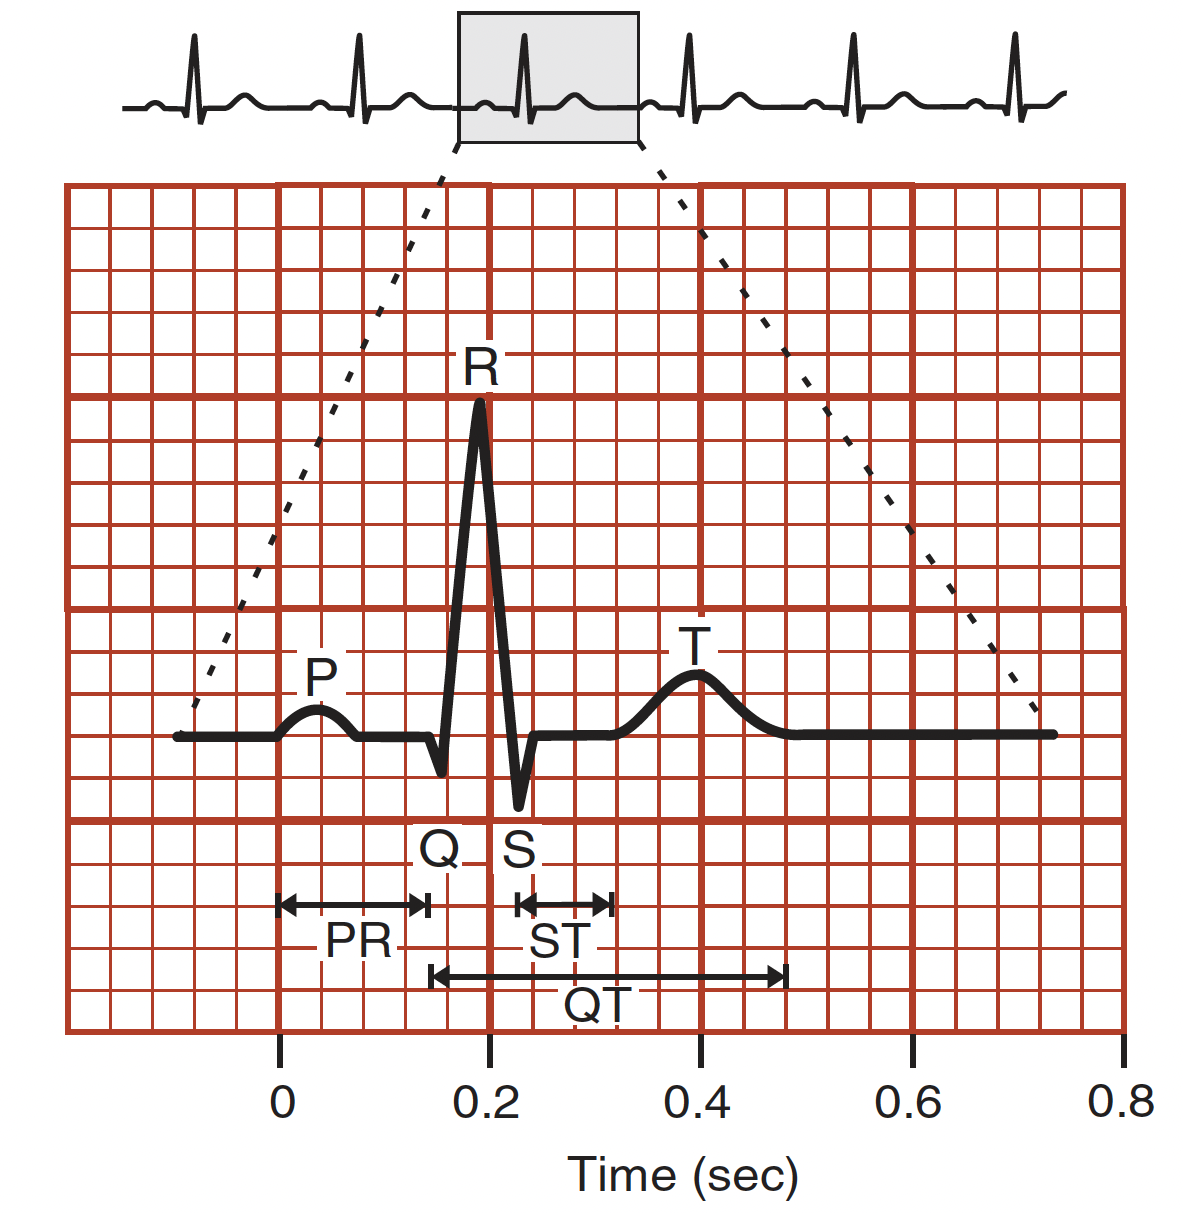
\includegraphics[width=1\linewidth]{images/ecg.png}
\caption{Components of the ECG trace. An enlargement of one of the repeating waveform units in the rhythm strip shows the P wave, QRS complex, and T wave, which represent atrial depolarization, ventricular depolarization, and ventricular repolarization, respectively. The PR interval represents the time required for the depolarization wave to transverse the atria and the AV node; the QT interval represents the period of ventricular depolarization and repolarization; and the ST segment is the isoelectric period when the entire ventricle is depolarized. Each small square is 1 mm. (\cite{alma991000225790601591})}
\label{fig:r-peaks}
\end{figure}

A 12-Lead ECG (Electrocardiogram) is a standard diagnostic tool used to assess the electrical activity of the heart. It provides a comprehensive view of the heart's electrical activity from different angles. The 12 leads consist of:

\begin{itemize}
  \item 6 precordial leads (V1-V6) placed on the chest
  \item 3 limb leads (I, II, III)
  \item 3 augmented limb leads (aVR, aVL, aVF)
\end{itemize}

% Each lead records the heart's electrical activity from a different perspective, providing information on:

% \begin{itemize}
%   \item Heart rate and rhythm
%   \item Conduction abnormalities
%   \item Chamber enlargement
%   \item Myocardial ischemia or infarction
%   \item Electrolyte imbalances
% \end{itemize}

The ECG machine typically records data for about 10 seconds, producing a graph of voltage versus time.

% The Electrocardiogram (ECG) is a crucial diagnostic tool in cardiology that records the electrical activity of the heart. A standard 12-lead ECG system provides multiple perspectives of cardiac electrical activity, facilitating comprehensive analysis.

% Signal Acquisition: ECG data is acquired through electrodes placed on the body surface, measuring potential differences over time.
% Waveform Components: The ECG waveform consists of P, Q, R, S, and T waves, each representing specific cardiac events.
% Lead System: The 12-lead system comprises:

% 6 precordial leads (V1-V6)
% 3 limb leads (I, II, III)
% 3 augmented limb leads (aVR, aVL, aVF)

add images sources

\begin{figure}[h!]
    \centering
    \subfigure{
        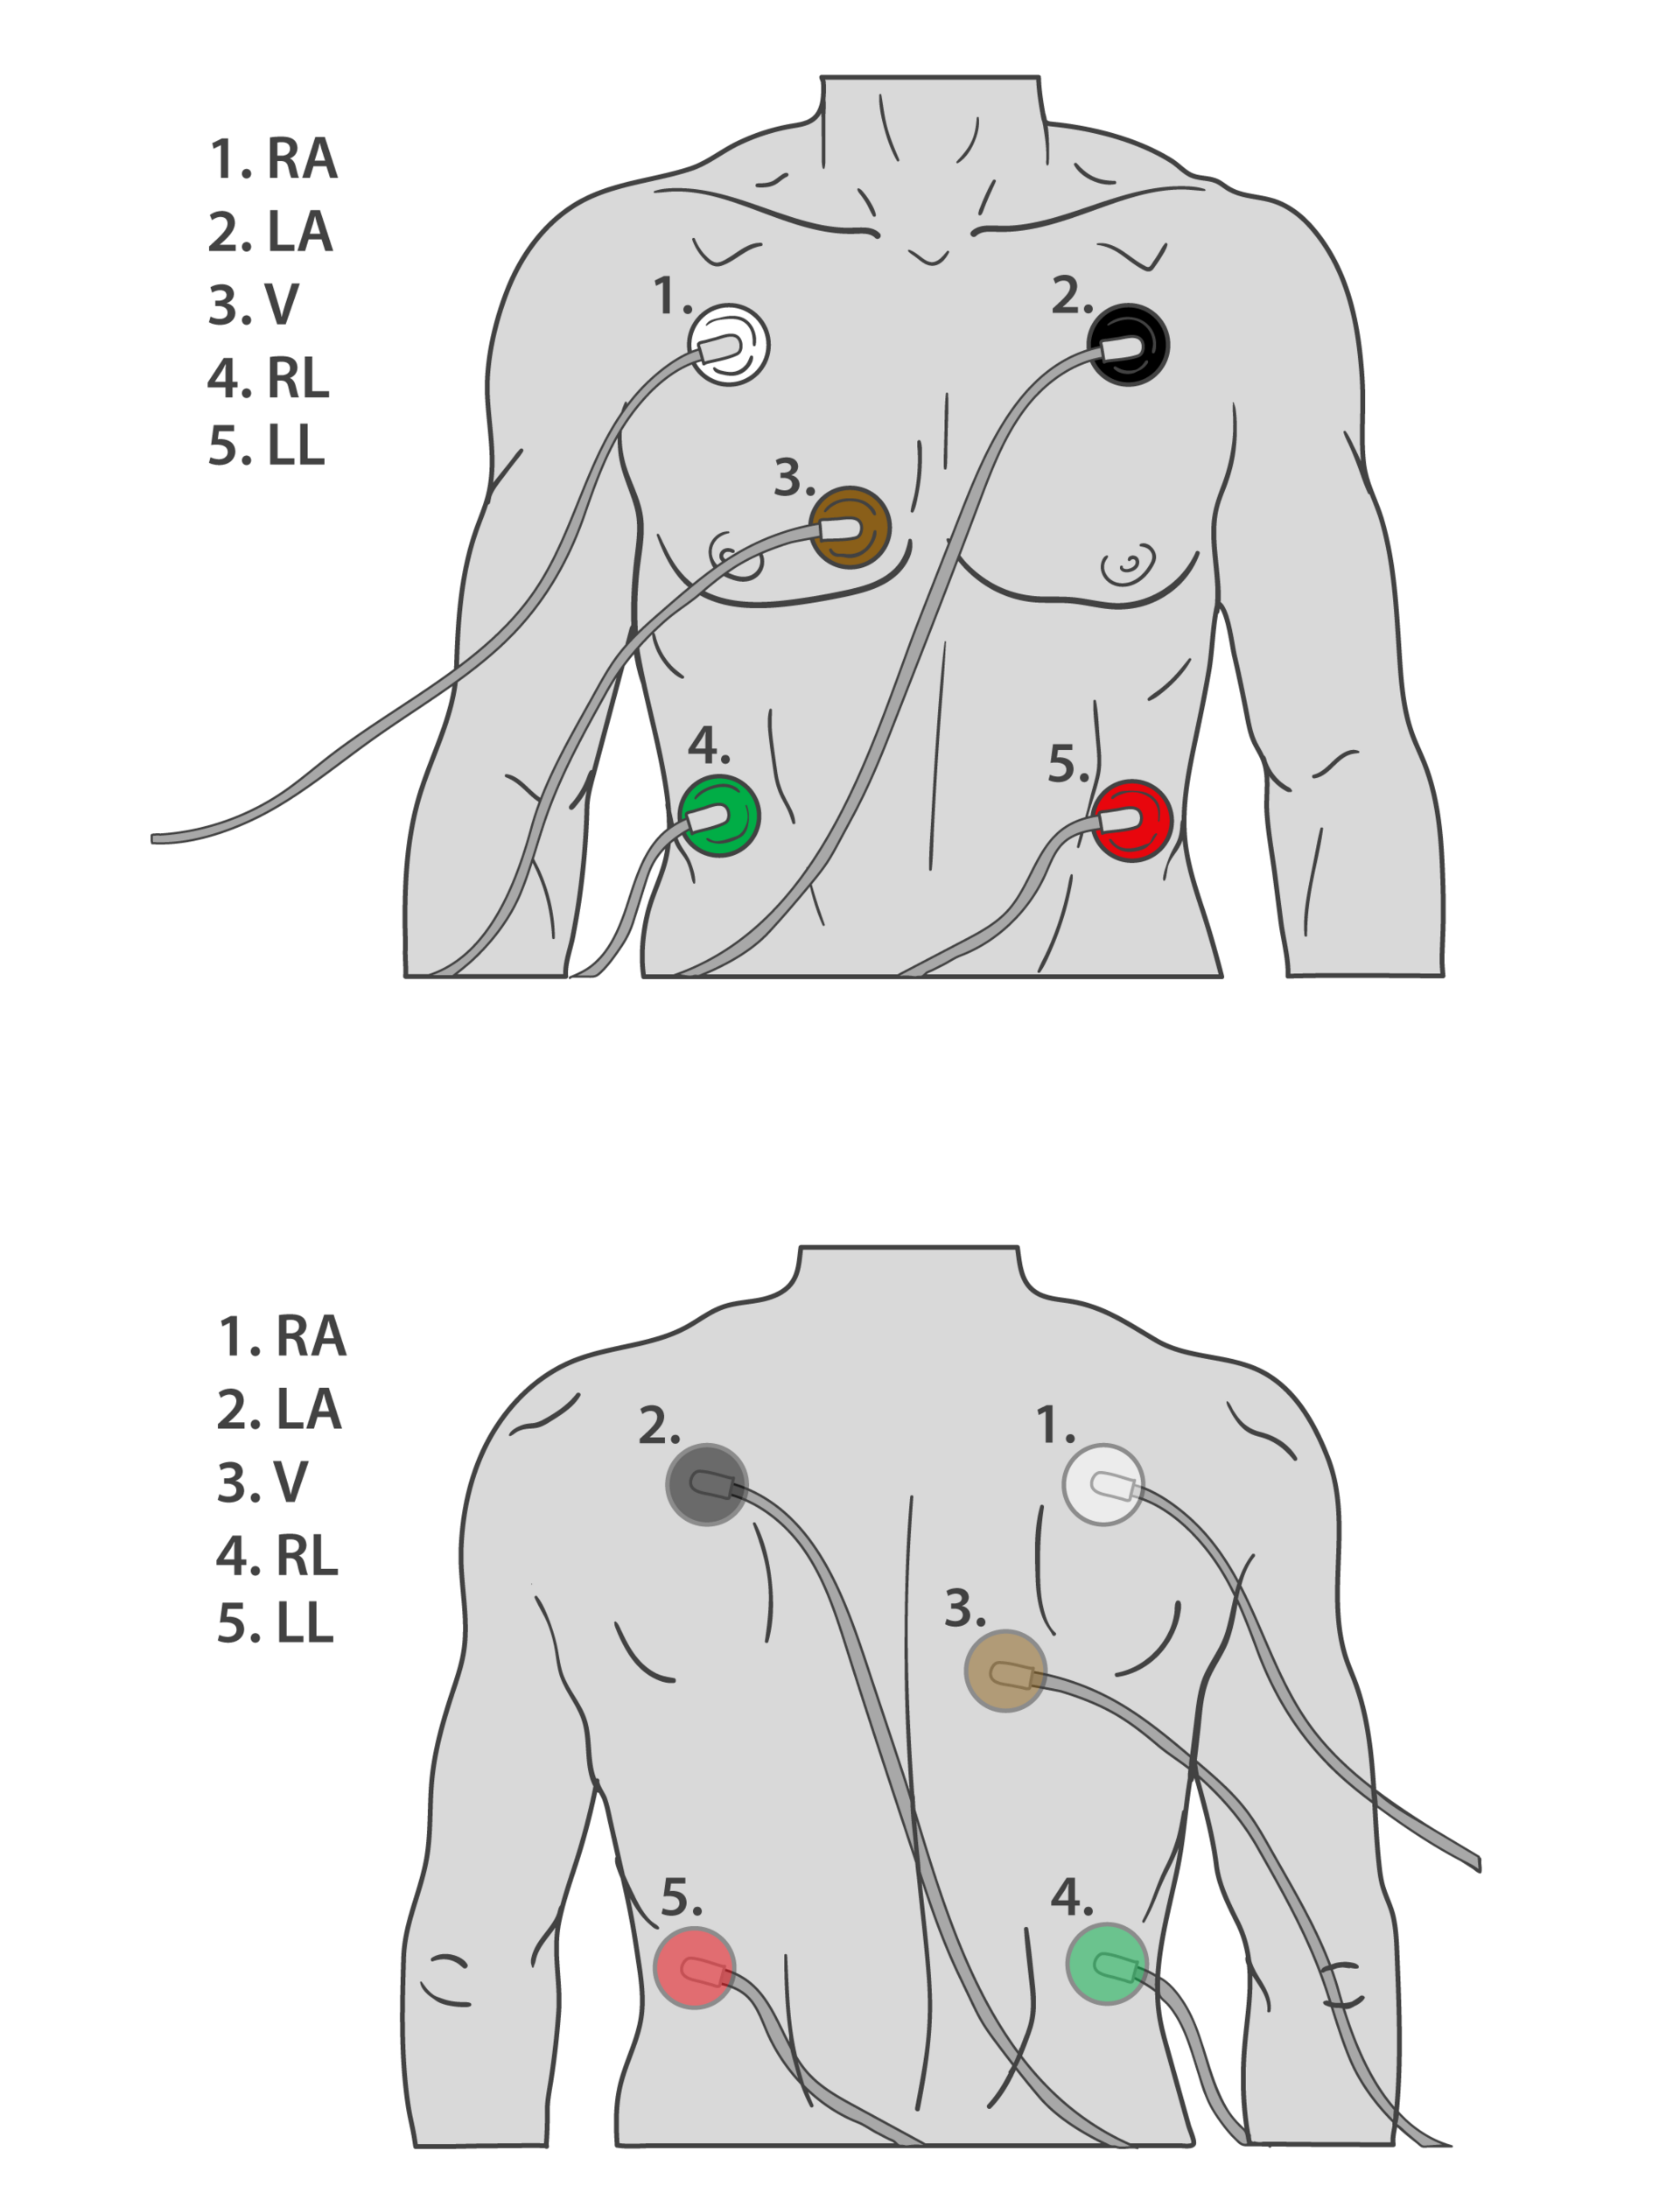
\includegraphics[width=0.48\linewidth]{images/ECG_Electrode_Placement.png}
        \label{fig:ecg-electrode}
    }
    \hfill
    \subfigure{
        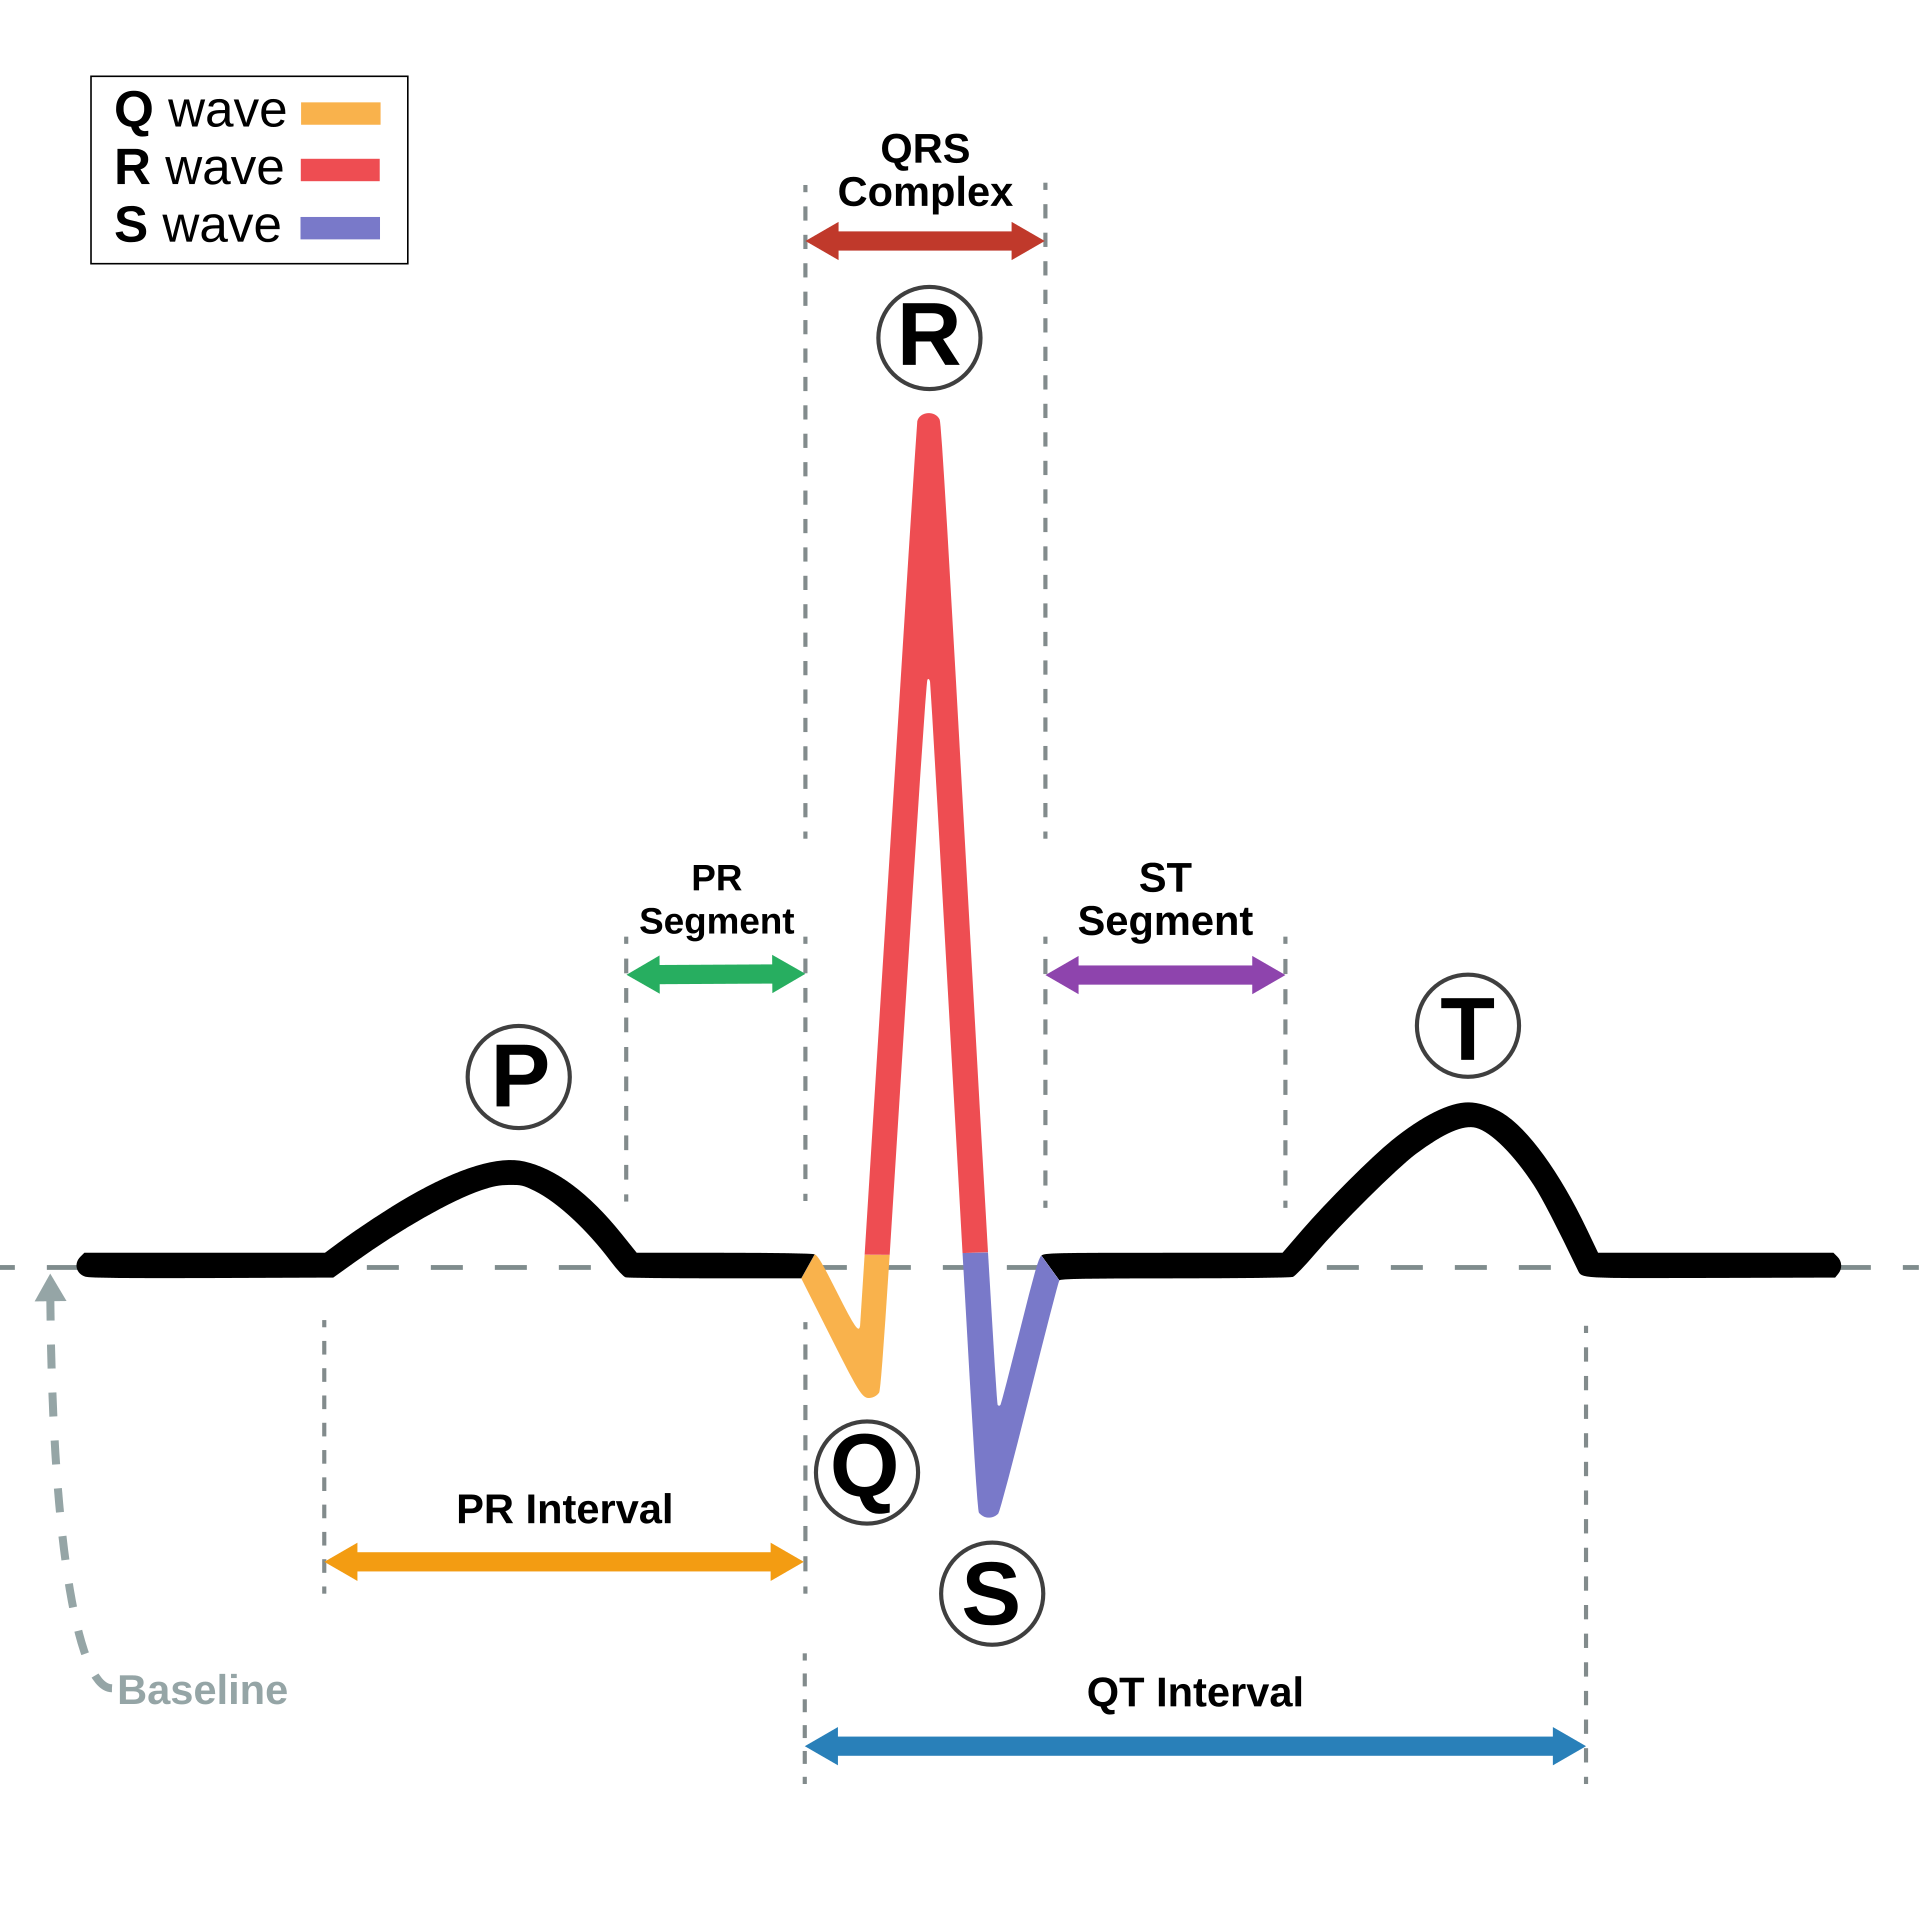
\includegraphics[width=0.48\linewidth]{images/SinusRhythmLabels.png}
        \label{fig:sinus-rhythm}
    }
    \caption{Left: . Right: }
    \label{fig:combined}
\end{figure}

TODO:

\begin{itemize}
    \item introduce PQRST
    \item mention R-peaks and their importance
    \item general information about the 12-leads 
    \item add images for ECG, leads placements, sources
\end{itemize}

% forcing a page break
\clearpage

\chapter{Experiments and Results}

The research aims to use the already available A Large Scale 12-lead Electrocardiogram Database for Arrhythmia Study (\cite{cite1}, \cite{cite2}, \cite{cite3}). This is a comprehensive database of high-quality 12-lead ECG signals collected from 45,152 patients. Each signal is with length of 10 seconds corresponding to 5000 data points. The dataset is designed to support arrhythmia research, containing labeled data for various cardiac conditions such as atrial fibrillation, premature ventricular contractions, and bundle branch blocks. This large dataset has high-quality labels from professional experts, diverse arrhythmia types, and additional cardiovascular conditions, making it suitable for performing different research tasks on it without spending time on gathering, cleaning and processing data. \newline


% • Presents a comprehensive database of 12-lead ECG signals collected from 45,152 patients. Each signal is with length of 10 seconds corresponding to 5000 data points.
% • The dataset is designed to support arrhythmia research, containing labeled data for various cardiac conditions such as atrial fibrillation, premature ventricular contractions, and bundle branch blocks.
% • ECG data is non-invasive and critical for diagnosing cardiovascular conditions, but analyzing such large
% datasets requires efficient automated methods.
% • Large dataset, high-quality labels from professional experts, diverse arrhythmia types, and additional cardiovascular conditions. \newline


% Pre,post, processing

% What exactly is tested - 5k points, sample from the points, results, smoothing, no smoothing, differеnt ranks, fourier terms

\section{Missing Data Imputation}

TODO:
\begin{itemize}
    \item data used - processing
    \item algorithms tested: psmf, rpsmf, mle-smf, tmf
    \item coverage, results
    \item add figures showing the original data, missing parts and imputed parts
\end{itemize}

%% DO NOT EDIT - AUTOMATICALLY GENERATED FROM RESULTS!
%% This table requires booktabs and multirow!
%% Table for missing percentage 20
\begin{table}[H]
    \centering
    \begin{threeparttable}
        \begin{tabular}{lccc}
            \hline
             & 20\% & 30\% & 40\% \\
            \hline
            PSMF & 0.39 & 0.32 & 0.24 \\
            rPSMF & \textbf{0.85} & \textbf{0.78} & \textbf{0.71} \\
            MLE-SMF & 0.18 & 0.16 & 0.15 \\
            \hline
        \end{tabular}
        \caption{Average coverage proportion of the missing data by the $2\sigma$ uncertainty bars of the posterior predictive estimates, averaged over 100 repetitions.}
    \end{threeparttable}
\end{table}

\begin{table}[H]
\centering
\label{tab:my_label}
\begin{tabular}{@{}lccc|ccccc@{}}
\toprule
 & \multicolumn{3}{c}{Imputation RMSE} & \multicolumn{3}{c}{Runtime (s)} \\
 & 20\% & 30\% & 40\% & 20\% & 30\% & 40\% \\
\midrule
PSMF & $\underset{{\scriptscriptstyle \;\;(20.80)}}{63.93}$ & $\underset{{\scriptscriptstyle \;\;(22.15)}}{80.90}$ & $\underset{{\scriptscriptstyle \;\;\;(21.30)}}{104.68}$ & 1.05 & 1.25 & 1.19 \\
rPSMF & $\underset{{\scriptscriptstyle \;\;(17.29)}}{\textbf{60.58}}$ & $\underset{{\scriptscriptstyle \;\;(18.50)}}{\textbf{74.56}}$ & $\underset{{\scriptscriptstyle \;\;(20.12)}}{\textbf{93.22}}$ & 1.22 & 1.31 & 1.17 \\
MLE-SMF & $\underset{{\scriptscriptstyle \;\;\;(22.15)}}{255.87}$ & $\underset{{\scriptscriptstyle \;\;\;(67.00)}}{263.76}$ & $\underset{{\scriptscriptstyle \;\;\;(81.31)}}{271.45}$ & 6.17 & 1.00 & 1.12 \\
TMF & $\underset{{\scriptscriptstyle \;\;\;(15.78)}}{169.83}$ & $\underset{{\scriptscriptstyle \;\;\;(16.33)}}{167.91}$ & $\underset{{\scriptscriptstyle \;\;\;(17.91)}}{155.58}$ & 2.11 & 0.50 & 0.58 \\
\bottomrule
\end{tabular}
\caption{Imputation error and runtime using 20\%, 30\% and 40\% missing values, averaged over 100 random repetitions.}
\end{table}

\section{R-peaks Detection}

TODO:
\begin{itemize}
    \item intro: why it is an important task, mention current methods?
    \item introduce the idea: smoother peaks, remove reconstruction from the original data
    \item threshold
    \item (potential) issues, improvements, results
    \item figure caption, more result figures
\end{itemize}

\begin{figure}[H]
\centering
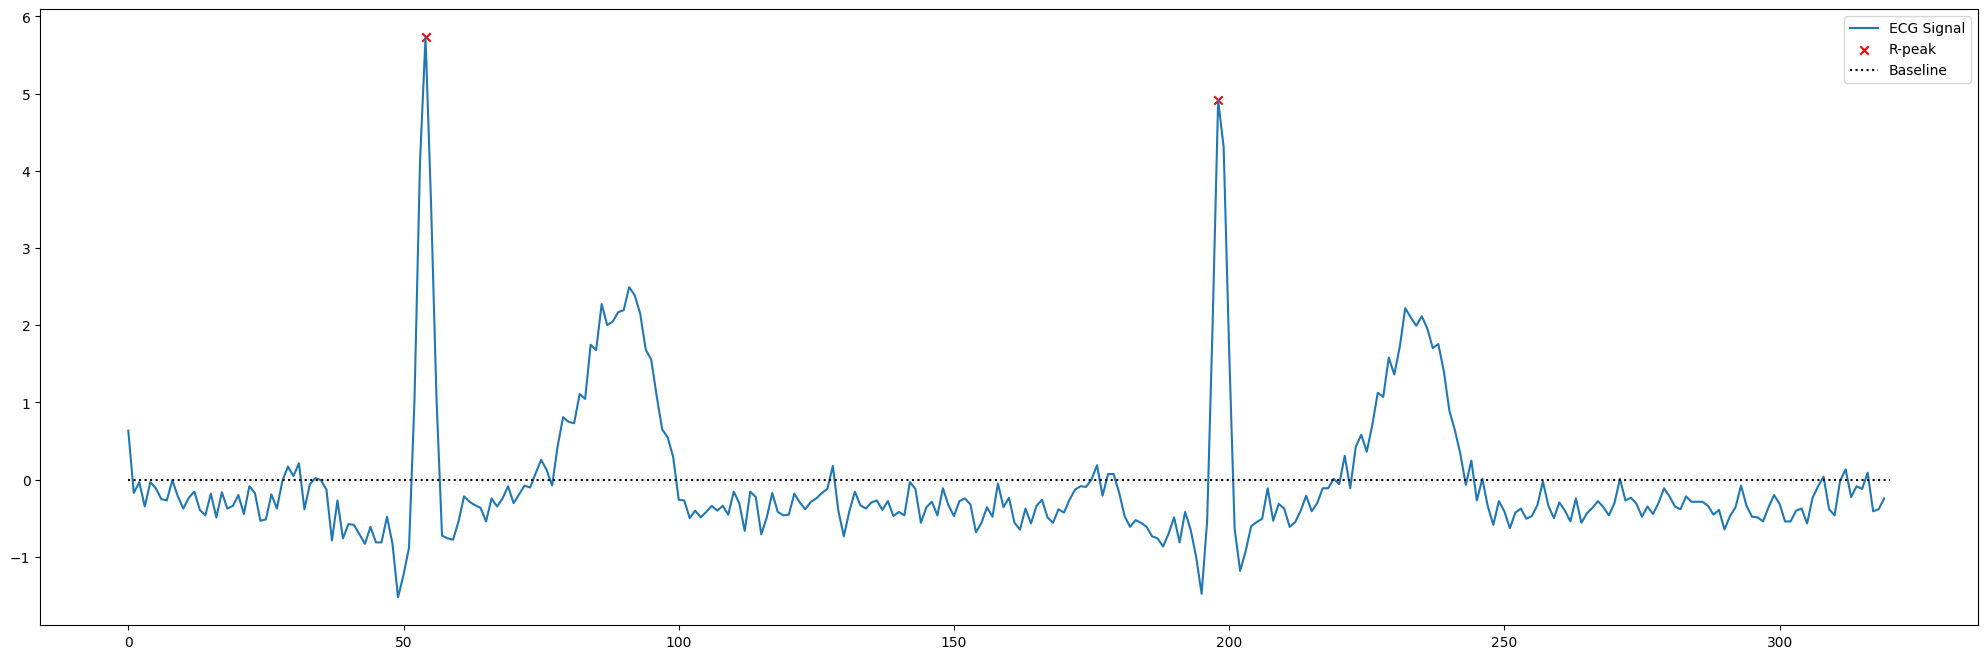
\includegraphics[width=1\linewidth]{images/r_peaks.png}
\label{fig:r-peaks}
\end{figure}

\section{Forecasting}

TODO:

\begin{itemize}
    \item original data (5000) vs subsample (1500)
    \item smoothing vs no smoothing
    \item Fourier basis and number of terms, higher rank
    \item encountered issues, conclusions
    \item add figures for the basis, loss curves, forecast (show different experiments results)
\end{itemize}

\begin{figure}[H]
\begin{center}
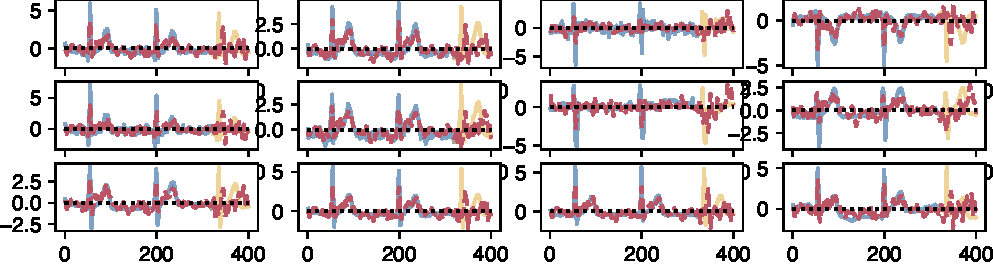
\includegraphics[scale=1]{images/periodic_fit_1500_6_6_150it.pdf}
\caption{My caption here}
\label{somelabelforreference}
\end{center}
\end{figure}

\chapter{Conclusion}

TODO: summarise results

\section{Future work}

TODO:
\begin{itemize}
    \item More complex model to better suit the complexity of the ECG data
    \item Better computational efficiency
\end{itemize}

\clearpage
 %% reset page counter and start appendix pages with A
\pagenumbering{arabic}
\renewcommand*{\thepage}{A\arabic{page}}

%% Appendix goes here
%\appendix
%
%\chapter{Appendix title}
%
%Appendix goes here.


%%References part of appendices
% References: modify the file refs.bib
\bibliographystyle{plainnat}
\bibliography{refs}


\end{document}
